\documentclass{article}
\title{Graph Algorithms}
\author{Christian Garcia}

\usepackage{graphicx}
\usepackage{hyperref}

\begin{document}

\maketitle

%\vspace{36pt} % 3 lines

\begin{Huge}
\section*{Questions}
\end{Huge}

\begin{figure}[!h]
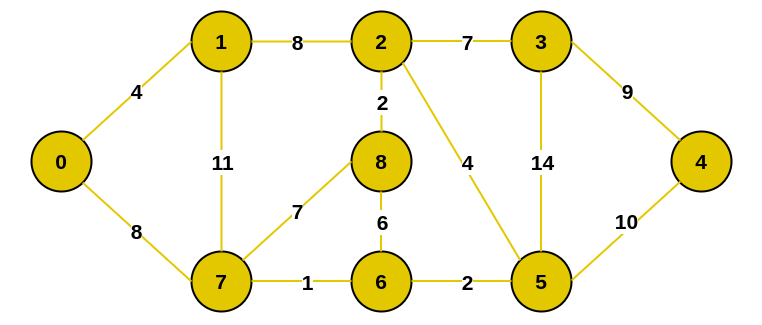
\includegraphics[width=\linewidth]{kruskalgraph.png}
\caption{Graph we are using for Kruskal's algorithm} Link: \href{https://www.javatpoint.com/cpp-dijkstra-algorithm-using-priority-queue}{https://www.javatpoint.com/cpp-dijkstra-algorithm-using-priority-queue}
\end{figure}

\subsection{Using the graph above, find the shortest path using Kruskal's algorithm. Please list the total cost to get from point 0 to point 8. Be sure to trace your steps when needed. }

\pagebreak{}

\subsection{Using the code from the link below, insert the graph into the adjacency matrix provided when you run the code. Compare the total cost to the handwritten version of Kruskal's algorithm. Copy and paste or download the code from this link: \href{https://github.com/ehawkvu/ds-n-a/blob/master/graphing/kruskal.c}{kruskal.c}.}

\vspace{36pt}

\begin{figure}[!h]
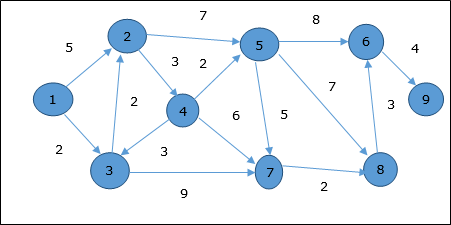
\includegraphics[width=\linewidth]{dijkstragraph.jpg}
\caption{Graph we are using for Dijkstra's algorithm} Link: \href{https://amogh-chothe18.medium.com/minimum-spanning-tree-algorithm-78fa9a7a707f} {https://amogh-chothe18.medium.com/minimum-spanning-tree-algorithm-78fa9a7a707f}
\end{figure}

\subsection{Using the graph above, find the shortest path using Dijkstra's algorithm. Use the table commonly associated with Dijkstra's algorithm as a proof of work.}

\pagebreak{}

\subsection{Using the code from the link below, modify the adjacency array to create the graph above. Compare the distances to your chart. Copy and paste or download the code from this link: \href{https://github.com/ehawkvu/ds-n-a/blob/master/graphing/dijkstra.c}{dijkstra.c}.}

\vspace{36pt}

\subsection{Modify both Dijkstra's algorithm and Kruskal's algorithm track the elapsed run time for each. How do the algorithms compare performance wise? Why do you think this is?}

\end{document}